\section{Theorie}
\label{sec:Theorie}
In diesem Abschnitt werden die theoretischen Grundlagen erläutert, die für den Versuch relevant sind.
%
%
%
%
%
\subsection{Stehende Wellen in einem Zylinder-Resonator}
Es soll zuerst ein Zylinderförmiger Resonator betrachtet werden, in dem sich akustische stehende Wellen ausbilden.
Entlang der $z$-Achse des Zylinders können diese stehenden Wellen als eindimensionale stehende Wellen angenommen werden.
Diese ergeben sich, wenn die einlaufende Welle an beiden Enden reflektiert wird. 
Es ergibt sich eine Überlagerung der reflektierten Wellen, sodass sich periodisch Knoten und Bäuche ergeben, wie es in \autoref{fig:stehendewelle} deutlich wird.  
Dabei sind bei einer gegebenen Länge $L$ des Resonators nur diskrete Wellenlängen $\lambda_n$ für die stehenden Wellen möglich. 
Für diese gilt die Bedinung \cite[405 f.]{demtröder_2021}
\begin{equation}
    \lambda_n = \frac{2 L}{n} \, . \nonumber
\end{equation}
Mit $\lambda = \frac{c}{f}$ ergibt sich damit für die Schallgeschwindigkeit $c$
\begin{equation}
    c = \frac{2 L f}{n} \, .
    \label{eqn:schallgeschw}
\end{equation}
Dabei ist $f$ die Frequenz der stehenden Welle.
\begin{figure}
    \centering
    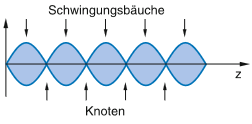
\includegraphics[width=0.3\textwidth]{content/images/stehendewelle.png}
    \caption{Darstellung einer eindimensionalen Stehenden Welle mit Knoten und Bäuchen~\cite[405]{demtröder_2021}.}
    \label{fig:stehendewelle}
\end{figure}
\FloatBarrier\noindent
%
%
%
%
%
%
%
\subsection{Stehende Wellen in einem Kugel-Resonator}
Nun sollen ein Kugelresonator betrachtet werden. 
Dreidimensionale akustische Wellen werden durch die Helmholtz-Glechung
\begin{equation}
    \increment p\left(\vec{r}\right) + k^2 p\left(\vec{r}\right) = 0 
\end{equation}
mit der Wellenzahl $k=\frac{2\pi}{\lambda}\frac{\omega}{c}$ beschrieben. %Quelle?
Dabei ist $\omega$ die Kreisfrequenz der Welle. 
Für den Kugelresonator sind Kugelkoordinaten $r$, $\vartheta$ und $\varphi$ die geeignete Wahl.
Damit ergibt sich als Lösung durch Seperation
\begin{equation}
    p = Y\left(\vartheta, \varphi\right)\cdot R\left(r\right) \, .
\end{equation}
Wobei $R\left(r\right)$ die Besselfunktionen, die die Gleichung 
\begin{equation}
    R''\left(r\right) + \frac{2}{r} R'\left(r\right)+ \left[k^2 - \frac{l\left(l+1\right)}{r^2}\right]R\left(r\right) = 0
\end{equation}
erfüllen, und $Y\left(\vartheta, \varphi\right)$ die Kugelflächenfunktionen
%\begin{equation}
%    \left[\frac{\partial^2}{\partial \vartheta^2} + \frac{\mathrm{cos}\vartheta}{\mathrm{sin}\vartheta}\frac{\partial}{\partial \vartheta} + \frac{1}{\mathrm{sin}^2 \varphi}\frac{\partial^2}{\partial \varphi^2} + l\left(l+1\right)\right]Y\left(\vartheta, \varphi\right) = 0
%\end{equation}
%erfüllen, sind.
\begin{equation}
    Y\left(\vartheta, \varphi\right) = \frac{1}{\sqrt{2 \pi}}N_{l,m} P_{l,m} \left(\mathrm{cos}\vartheta\right) \mathrm{e}^{\mathrm{i}m \varphi}
\end{equation}
sind. Dabei sind $l$ und $m$ die Seperationskonstanten, $N_{l,m}$ ist ein Normierungsfaktor und $P_{l,m}$ sind die zugeordneten Legendrepolynome \cite{ehlotzky_2007}.
%Es ergibt sich 
%\begin{equation}
%     p\left(r, \vartheta, \varphi\right)= \sum_{l=0}^\infty \sum_{m=-l}^{+l} \frac{1}{\sqrt{kr}}\left( A_{l,m} R_{l+\frac{1}{2}}\left(kr\right) + B_{l,m} R_{-\left(l+\frac{1}{2}\right)}\left(kr\right)\right) P_l^m \left(\mathrm{cos}\vartheta\right) \mathrm{e}^{\mathrm{i}m \varphi}
%\end{equation}
%Dabei handelt es sich bei $l$ und $m$ um Seperationskonstanten.
%Außerdem sind $P_l^m$ die zugeordneten Legendrepolynome sind.
%
%
%
\subsection{Relative Abweichung experimenteller Messwerte}
Zur Berechnung der relativen Abweichung von experimentell bestimmten Werten zu theoretischen Werten wird 
\begin{equation}
    \increment x_{\mathrm{rel}} = \left| \frac{x_{\mathrm{\exp}}-x_{\mathrm{theo}}}{x_{\mathrm{theo}}}\right|
    \label{eqn:relabw}
\end{equation}
verwendet~\cite{relabw}. 

